\documentclass[11pt]{article}
\usepackage[hmargin=1in,vmargin=1in]{geometry}
\usepackage{xcolor}
\usepackage{amsmath,amssymb,amsfonts,url,sectsty,framed,tcolorbox,framed}
\usepackage{nicematrix}
\setcounter{MaxMatrixCols}{16}
\usepackage{tikz}
\usepackage{hyperref}
\usetikzlibrary{decorations.pathreplacing}
\newcommand{\pf}{{\bf Proof: }}
\newtheorem{theorem}{Theorem}
\newtheorem{lemma}{Lemma}
\newtheorem{proposition}{Proposition}
\newtheorem{definition}{Definition}
\newtheorem{remark}{Remark}
\newcommand{\qed}{\hfill \rule{2mm}{2mm}}


\begin{document}
%%%%%%%%%%%%%%%%%%%%%%%%%%%%%%%%%%%%%%%%%%%%%%%%%%%%%%%%%%%%%%%%%%%%%
\noindent
\rule{\textwidth}{1pt}
\begin{center}
{\bf [CS304] Introduction to Cryptography and Network Security}
\end{center}
Course Instructor: Dr. Dibyendu Roy \hfill Winter 2022-2023\\
Scribed by: Archit Agrawal (202051213) \hfill Lecture 8 and 9 (Week 5)
\\
\rule{\textwidth}{1pt}
%%%%%%%%%%%%%%%%%%%%%%%%%%%%%%%%%%%%%%%%%%%%%%%%%%%%%%%%%%%
%write here

\section{Quick Recap}
In Week 4, the following topics were covered:
\begin{itemize}
    \item Attack Models (Cipher Text Only, Known Plaintext, Chosen Plaintext, Chosen Ciphertext) 
    \item Cryptanalysis of DES
    \item Double and Triple Encryption of DES
    \item Mathematics Recall (Group, Abelian Group and Finite Group)
\end{itemize}

\section{Generators and Cyclic Group}
Consider a group $(G, *)$. Let $\alpha \in G$. The identity element $\alpha^0$ belongs to G. Therefore,
\begin{center}
    $\alpha^0 * \alpha = \alpha^1$\\
    \vspace{1mm}
    $\alpha^1 * \alpha = \alpha^2$\\
    \vspace{1mm}
    $\alpha^2 * \alpha = \alpha^3$\\
\end{center}
Keep in mind, the $*$ here is not multiplication, it is a binary operation not necessarily multiplication. $\alpha^1, \alpha^2, \alpha^3$ and so on, are just notation of using the binary operation $*$ on same element. Since, G is closed under $*$, any two elements belonging to G, will give the result in G on performing the binary operation $*$. Since $\alpha^0 \in G$ and $\alpha \in G$, therefore $\alpha^1 \in G$. Now, since $\alpha^1 \in G$, therefore $\alpha^2 \in G$, and so on. That means,
\begin{center}
    $\alpha^0, \alpha^1, \alpha^2, ... \in G$
\end{center}
The set $\alpha^0, \alpha^1, \alpha^2, ...$ is denoted by $\langle \alpha \rangle$. Also, $\langle \alpha \rangle \subseteq G$. $\alpha$ is called the generator of $(G, *)$ iff:
\begin{center}
    for any $b \in G$ $\exists$ $i \geq 0$ such that $b = \alpha^i$
\end{center}
A group is called a cyclic group if there is an element $\alpha \in G$, such that for every $b \in G$, there is an integer $i$ with $b = \alpha^i$.


\section{Subgroup of a Group}
Let $(G, *)$ be a finite group. Let $a \in G$ and $O(a)$ be the order of $a$. The order of an element $a$ is defined as the least positive integer $m$ such that $a^m$ is identity element $e$. Therefore,
\begin{center}
    $O(a) = m$\\
    and, $a^m = e$
\end{center}
Now, $a^{m+1} = a, a^{m+2} = a^2$ and so on, that is, after $a^{m-1}$, all elements will be repeated.\\
\newline
Hence, the set $H = \{e = a^0, a^1, a^2,....., a^{m-1}\}$ will be finite and will have the following properties:

\begin{enumerate}
    \item $H \subseteq G$
    \item H is a group under $*$.
    \begin{itemize}
        \item It has identity element $a^0$.
        \item G is associative on $*$ and $H \subseteq G$, therefore, H is associative on $*$.
        \item H is closed under $*$ as each element is of the form of $a^x$. Therefore, for two elements $a^i$ and $a^j$, $a^i * a^j = a^{i+j}$. If $(i + j) < m$, $a^{i+j}$ is clearly in H, otherwise, if $(i+j)$ exceeds $(m-1)$, the values are repeated as we discussed above.
        \item For each $a^i$ in H, inverse $a^{m-i}$ exists in H.
    \end{itemize}
\end{enumerate}
Such a group H is called a subgroup of G. Also, H is cyclic because its elements can be generated from only anyone element belonging to H. \textbf{Every group has always a cyclic subgroup}. Also, the order of the element is equal to the cardinality of the generated cyclic subgroup.
\begin{center}
    $|H| = |\langle a \rangle|$ = order of cyclic group
\end{center}

\section{Lagrange's Theorem}
If G is a finite group and H is a subgroup of G, then $|H|$ divides $|G|$. Since, the order of the element generating the subgroup is equal to the cardinality of the subgroup, therefore, order of the element also divides $|G|$. Let $a \in G$ and $O(a)$ be order of element a. Therefore, 
\begin{center}
    $H = \{a^0, a^1, a^2,....,a^{O(a)-1} \}$
\end{center}
From Lagrange's Theorem, 
\begin{center}
    $|H|$ divides $|G|$ $\implies$ $O(a)$ divides $|G|$
\end{center}

\subsection{Few results}
\begin{itemize}
    \item If order of $a \in G$ is t, then order of $a^k$ is $\frac{t}{gcd(t, k)}$.
    \item If gcd(t, k) = 1, then $O(a^k) = t = O(a)$. This implies that $|\langle a^k \rangle| = |\langle a \rangle|$. Assume an element $x \in \langle a^k \rangle$.
    \begin{center}
        $x = (a^k)^i = a^{ki} \in \langle a \rangle$
    \end{center}
    This means that $\langle a^k \rangle$ and $\langle a \rangle$ are equal sets.

    \item The above points conclude that $a^k$ is a generator of cyclic group $\langle a \rangle$ iff $k$ is co-prime to $O(a)$.
\end{itemize}

\textbf{Example:} Consider the set $Z_{19}^* = \{x | gcd(x,19) = 1, 1 \leq x \leq 18\}$ and $*_{19}$ be the operation multiplication modulo 19. Find generators of $(Z_{19}^*, *_{19})$.\\
\textbf{Solution:} Take $x \in Z_{19}^*$ and compute $\langle x \rangle$.
\begin{center}
    $\langle 2 \rangle = \{1,2,4,8,16,13,7,14,9,18,17,15,11,3,6,12,5,10\}$
\end{center}
Clearly, we can see 2 is generator of $Z_{19}^*$ under $*_{19}$. The order of 2 is 18. Now, to find other generators of $Z_{19}^*$, we need to find k such that k is co-prime to 18. Other generators will be $2^k$ (k is not exponent here, it is the $*_{19}$) operation. Since, 2, 3, 4 are not co-prime to 18, hence, 4, 8, 16 are not generators of $Z_{19}^*$. Since, 5 is co-prime to 18, hence, $2^5 = 13$ is a generator of $Z_{19}^*$. Similarly, 14, 15, 3 and 10 are generators of $Z_{19}^*$.

\section{Ring}
A ring $(R, +_R, \times_R)$ consists of one set R with two binary operations arbitrarily denoted by $+_R$ (addition) and $\times_R$ (multiplication) on R satisfying the following properties:
\begin{enumerate}
    \item $(R, +_R)$ is an abelian group with the identity element $0_R$.
    \item The operation $\times_R$ is associative, that is, 
    \begin{center}
        $a \times_R (b \times_R c) = (a \times_R b) \times_R c$ for all $a, b, c \in R$
    \end{center}
    \item There is a multiplicative identity denoted by $1_R$ with $1_R \neq 0_R$ such that $1_R \times_R a = a \times_R 1_R = a$ for all $a \in R$.
    \item The operation $\times_R$ is distributive over $+_R$, that is,
    \begin{center}
        $(b +_R c) \times_R a = (b \times_R a) +_R (c \times_R a)$\\
        $a \times_R (b +_R c) = a \times_R b + a \times_R c$
    \end{center}
\end{enumerate}

\textbf{Example:} Is $(Z, +, \cdot)$ a ring or not?\\
\textbf{Solution:} Since, addition on integers is both commutative and associative, also the identity element exists (0) and additive inverse for each elements exists (-a). Hence, $(Z, +)$ is an abelian group. Also, since, multiplication on integers is associative and distributive over addition and each integer can be multiplied by identity element 1 (which is not same as additive identity). Therefore, $(Z, +, \cdot)$ is a ring.\\

\textbf{Example:} Is $(R, +, \cdot)$ a ring or not?\\
\textbf{Solution:} Similar to previous example, it can be proved that $(R, +)$ is an abelian group. Also, multiplication is both associative and distributive over real numbers. The identity element for multiplication is 1 for real numbers. Hence, $(R, +, \cdot)$ is a ring.\\

\textbf{Example:} Is $(Z_n, +_n, *_n)$ a ring or not?\\
\textbf{Solution:} In previous week lectures, we proved that $(Z_n, +_n)$ is an abelian group. Also, modular multiplication is both associative and distributive over integers. The identity element for multiplication is 1 for integers in $Z_n$. Hence, $(Z_n, +_n, *_n)$ is a ring.\\

If a ring is commutative under the second operation that is $\times_R$, it is called a commutative ring. It should also be noted that it is not necessary that inverse exists under the second operation.\\

An element 'a' of a ring R is called unit or an invertible element id there is an element $b \in R$ such that $a \times_R b = 1_R$. For example, for the ring $(Z, +, \cdot)$, the only unit element is 1. For the ring $(Z_n, +_n, *_n)$, all $x$ with gcd(x, n) = 1 are unit elements.

The set of units in a ring R forms a group under multiplication operation (second operation). This is known as group of units of R.

\section{Field}
A field is a non-empty set F together with two binary operations addition(+) and multiplication(*) for which the following properties are satisfied:
\begin{enumerate}
    \item $(F, +)$ is an abelian group
    \item If $0_F$ denotes additive identity element of $(F, +)$, then $(F - \{0_F\}, *)$ is a abelian group.
    \item For all $a,b,c \in F$, we have $a * (b + c) = (a * b) + (a * c)$
\end{enumerate}

\textbf{Example:} Is $(Z, +, \cdot)$ a field?\\
\textbf{Solution:} We know from previous examples that $(Z, +)$ is an abelian group with identity element 0. However, for the set $Z - \{0\}$, multiplicative inverse does not exist. Hence, $(Z - \{0\}, \cdot)$ is not an abelian group. Hence, $(Z, +, \cdot)$ is not a field.\\

\textbf{Example:} Is $(Q, +, \cdot)$ a field?\\
\textbf{Solution:} We know from previous examples that $(Z, +)$ is an abelian group with identity element 0. Also, for the set $Q - \{0\}$, multiplicative inverse exists for each rational number. Moreover, multiplication is distributive over addition on rational numbers. Hence, $(Q, +, \cdot)$ is a field.\\

\textbf{Example:} Is $(\mathbb{F}_p, +_p, *_p)$ a field, where p is a prime number?\\
\textbf{Solution:} We know that $(\mathbb{F}_p, +_p)$ an abelian group with identity element 0. Now, the set $\mathbb{F}_p - \{0\}$ has existing multiplicative inverse iff gcd(x, p) = 1 for each $x \in \mathbb{F}_p - \{0\}$. Since, p is prime, gcd(x, p) = 1 for all possible integers that $x$ can take. Hence, $(\mathbb{F}_p, +_p, *_p)$ is a field.\\


%Lecture 9 

\section{Field Extension}
Suppose $K_2$ is a field with addition(+) and multiplication(*). Suppose $K_1 \subseqeq K_2$ is closed under both these operations such that $K_1$ itself is a field with the restriction of + and * to the set $K_1$. Then $K_1$ is called a subfield of $K_2$ and $K_2$ is called a field extension of $K_1$.

\section{Polynomial Ring}
Let $(F, +, *)$ be a field and the set of polynomials of any degree $F[x]$ be:
\begin{center}
    $F[x] = \{a_0 + a_1\cdot x + a_2 \cdot x^2 +.... | a_i \in F\}$
\end{center}
$F[x]$ is set of all polynomials in $x$ with coefficients belonging to set F of the given field. The set of polynomials along with the binary operations of the field forms a ring and this ring is known as polynomial ring.

\begin{center}
    $(F[x], +, *) \rightarrow$ Polynomial Ring\\
    \vspace{1mm}
    $P_1(x) \in F[x] = a_0 + a_1 \cdot x +....+ a_n \cdot x^n$\\
    \vspace{1mm}
    $P_2(x) \in F[x] = b_0 + b_1 \cdot x +....+ b_n \cdot x^n$\\
\end{center}
If we want to add the two polynomials,
\begin{center}
    $P_1(x) + P_2(x) = (a_0 + a_1 \cdot x +....+ a_n \cdot x^n) + (b_0 + b_1 \cdot x +....+ b_n \cdot x^n)$\\
    \vspace{1mm}
    $P_1(x) + P_2(x) = (a_0 + b_0) + (a_1 + b_1) \cdot x +.....+ (a_n + b_n) \cdot x^n$
\end{center}
The coefficients $a_i, b_i$ belong to set F and the addition operation is the field addition of the field $(F, +, *)$. Since $(F, +, *)$ is a field, therefore, $(F, +)$ is an abelian group and addition on elements of F is closed. Therefore, $P_1(x) + P_2(x)$ is closed under addition because for any $i$, $(a_i + b_i) \in F$. Also, addition of polynomials is just coefficient-wise, hence, addition of polynomials will be associative because of field properties of coefficients. Similarly, the additive identity of field will be the additive identity of the polynomial in $F[x]$. Now, let's look at additive inverse of $P(x)$.
\begin{center}
    $P(x) = a_0 + a_1 \cdot x +.....+ a_n \cdot x^n$\\
    $P(-x) = -a_0 + (-a_1) \cdot x +.....+ (-a_n) \cdot x^n$\\
\end{center}
Clearly, $P(-x)$ is additive inverse of $P(x)$. Here, the negative sign does not mean the standard negation. It implies the additive inverse of $a_i$ in the field F. Also, 
\begin{center}
    $P_1(x) + P_2(x) = P_2(x) + P_1(x)$
\end{center}
Therefore, under addition the polynomial set $F[x]$ is an abelian group. Now, let's look at the multiplication operation of the two polynomials:
\begin{center}
    $P_1(x) * P_2(x) = (a_0 + a_1 \cdot x +....+ a_n \cdot x^n) * (b_0 + b_1 \cdot x +....+ b_n \cdot x^n)$\\
    \vspace{1mm}
    $P_1(x) * P_2(x) = (a_0 * b_0) + (a_0 * b_1 + b_0 * a_1) \cdot x +.....+ (a_n * b_n)\cdot x^n$
\end{center}
The multiplication operation is field multiplication operation and hence is associative, distributive. Also, the multiplicative identity also exists for the polynomials in $F[x]$. Hence, $(F[x], +, *)$ is a polynomial ring.

Let us define a polynomial ring formally. A set of polynomials $F[x]$ along with the operation of addition(+) and multiplication(*) is called a ring if:
\begin{enumerate}
    \item $(F[x], +)$ is an abelian group.
    \item * is associative over $F[x]$.
    \item An identity element over multiplication exists.
    \item * is distributive over +.
\end{enumerate}

\textbf{Example:} Consider the set $\mathbb{F} = \{0, 1\}$ and the field $(\mathbb{F}, +_2, *_2)$. Therefore, the polynomial set $\mathbb{F}_2[x]$ is:
\begin{center} 
    $\mathbb{F}_2[x] = \{a_0 + a_1 \cdot x + .... | a_i \in \mathbb{F}\}$
\end{center}
Let us just take two polynomials from this set:
\begin{center}
    $p(x) = x + 1$\\
    \vspace{1mm}
    $q(x) = x^2 + x + 1$\\
    \vspace{1mm}
    $p(x) +_2 q(x) = (x + 1) +_2 (x^2 + x + 1) = x^2 + (1 +_2 1) \cdot x + (1 +_2 1) = x^2$ \\
    \vspace{1mm}
    $p(x) *_2 q(x) = (x + 1) *_2 (x^2 + x + 1)$\\
    \vspace{1mm}
    $p(x) *_2 q(x) = (x^3 + x^2 + x) + (x^2 + x + 1) = x^3 + (1 +_2 1) \cdot x^2 + (1 +_2 1) \cdot x + 1$\\
    \vspace{1mm}
    $p(x) *_2 q(x) = x^3 + 1$
\end{center}

\section{Irreducible Polynomial}
A polynomial $P(x) \in F[x]$ of degree $n \geq 1$ is called irreducible if it cannot be written in the form of $P_1(x) * P_2(x)$ with $P_1(x), P_2(x) \in F[x]$ and degree of $P_1(x), P_2(x)$ must be greater than or equal to 1. It means that $P(x)$ is irreducible if it can not be factorised.\\
\newline
\textbf{Example:} $x^2 + 1 \in \mathbb{F}_2[x]$.\\
\textbf{Solution:} $(x + 1) * (x + 1) = x^2 + (1 + 1) \cdot x + 1 = x^2 + 1$. Therefore, $(x^2 + 1) =  (x + 1) * (x + 1)$ in $\mathbb{F}_2[x]$. Hence, $(x^2 + 1)$ is reducible in $\mathbb{F}_2[x]$. Note that it is not possible to factor $x^2 + 1$ in $\mathbb{R}[x]$, where $\mathbb{R}$ is set of real numbers.\\

\subsection{Ideal Generated by P(x)}
It is a set denoted by I which contains the polynomials given as:
\begin{center}
    $I = \langle P(x) \rangle = \{q(x) \cdot P(x) | q(x) \in F[x]\}$
\end{center}

Consider the set denoted by $F[x]/\langle P(x)  \rangle$ whose each element is formed by taking an element from $F[x]$ and then dividing it by $P(x)$. That is,
\begin{center}
    $q(x) \in F[x] = d(x) * P(x) + r(x)$\\
    \vspace{1mm}
    $r(x) \in F[x]/\langle P(x)  \rangle$
\end{center}
The remainder obtained belongs to the set $F[x]/\langle P(x)\rangle$. Now, if P(x) is irreducible polynomial, then $(F[x]/\langle P(x) \rangle, +, *)$ becomes a field. Here, the addition and multiplication operation are under modulo P(x). The degree of r(x) is always lesser than degree of P(x).\\

\textbf{Example:} $x^2 + x + 1 \in F_2[x], F_2 = \{0, 1\}$. $P(x) = x^2 + x + 1$ is irreducible.\\

Consider the set $F_2[x]/\langle x^2 + x + 1\rangle$:
\begin{center}
    $q(x) = d(x) \cdot P(x) + r(x)$\\
    $deg(r(x)) < 2$\\
    $r(x) = \{0, 1, x, x + 1\}$
\end{center}

If P(x) is a n degree polynomial under modulo 2, then there will be $2^n$ polynomials in r(x), that is, $F_2[x]/\langle x^2 + x + 1\rangle$.

Consider now for example a polynomial $X^2 + 1 \in F_2[x]$. Let's find the remainder on dividing it by P(x). For $F_2$, the remainder can be found in an easy way. It can be done by replacing $x^2$ in dividend with the lesser degree part of divisor, that is, $(x + 1)$. Therefore, 
\begin{center}
    $x^2 + 1 = q(x) * (x^2 + x + 1) + r(x)$\\
    $r(x) = x + 1 + 1 = x$
\end{center}

Let's take another example, say, $x^3 + 1$:
\begin{center}
    $x^3 + 1 = q(x) * (x^2 + x + 1) + r(x)$\\
    $r(x) = x \cdot x^2 + 1 = x \cdot (x + 1) + 1$\\
    $r(x) = x^2 + x + 1 = x + 1 + x + 1 = 0$
\end{center}
We saw that the remainder came out to be 0 and x. We can take other examples where the remainder will come out to be the remaining two polynomials, that are, 1 and $(x + 1)$.

\section{Primitive Polynomial}
Consider the set $F_2[x]/\langle x^2 + x + 1\rangle$. We have discussed that if the P(x) is irreducible then $(F[x]/\langle P(x) \rangle, +, *)$ becomes a field. Now, let's say if $\alpha$ is a root of $x^2 + x + 1 = 0$, that is,
\begin{center}
    $\alpha^2 + \alpha + 1 = 0$\\
    $\alpha^2 = -\alpha + (-1) = \alpha + 1$
\end{center}
If $\alpha$ can generate all the possible polynomials in $F_2[x]/\langle x^2 + x + 1\rangle$, then $x^2 + x + 1$ is known as primitive polynomial. Now, let's see:
\begin{center}
    $\langle \alpha \rangle = \{0, 1 = \alpha^0, \alpha, \alpha + 1 = \alpha^2\}$\\
    $O(\alpha) = 2$
\end{center}
Hence, $x^2 + x + 1$ is a Primitive Polynomial.\\

\textbf{Example:} $\mathbb{F}_2[x]/\langle x^3 + x + 1 \rangle$\\
\textbf{Solution:} The maximum number of polynomials that can be generated:
\begin{center}
    $\{0, 1, x, x + 1, x^2, x^2 + 1, x^2 + x, x^2 + x + 1\}$
\end{center}
Let's check if root of $x^3 + x + 1 = 0$ is a generator or not.
\begin{center}
    $\alpha^3 + \alpha + 1 = 0 \implies \alpha^3 = \alpha + 1$\\
    \vspace{1mm}
    $\langle \alpha \rangle = \{0, 1 = \alpha^0, \alpha, \alpha^2, \alpha + 1 = \alpha^3, \alpha^2 + \alpha = \alpha^4, \alpha^2 + \alpha + 1 = \alpha^5, \alpha^2 + 1 = \alpha^6\}$
\end{center}
Since, we are able to generate all the polynomials, therefore $x^3 + x + 1$ is a primitive polynomial. Note that there may exists a polynomial that is not a primitive polynomial but is still a field. That means, we will be able to find multiplicative inverse. Let us consider for the polynomial $x$. Instead of 1/x, we have a polynomial $x^2 + 1$, which will give 1 as result on multiplication.
\begin{center}
    $x * (x^2 + 1) = x^3 + x = x + 1 + x = 1$
\end{center}
Similarly, for $x^2$ the multiplicative inverse is $x^2 + x + 1$.
\begin{center}
    $x^2 * (x^2 + x + 1) = x^4 + x^3 + x^2 = x * (x + 1) + (x + 1) + x^2$\\
    $x^2 * (x^2 + x + 1) = x^2 + x + x + 1 + x^2 = 1$
\end{center}

\section{Advanced Encryption Standard}
When the design of DES was made public, it was immediately broken. Thereafter, NIST called for a competition named Advanced Encryption Standard. A lot of cryptographers around the world submitted their designs along with the implementation. One of the submission in the competition was $\emph{Rijndael}$. It was developed by two Belgian cryptographers, Joan Daemen and Vincent Rijmen. In the proposal, it was mentioned that the winner will be renamed as Advanced Encryption Standard. AES is unbreakable till date.\\

Advanced encryption Standard is an iterated block cipher and is based on Substitution Permutation Network(SPN). There are three different variants of AES:
\begin{enumerate}
    \item AES-128 (Block Size 128-bit, Number of Rounds = 10, Secret Key Size 128-bit)
    \item AES-192 (Block Size 128-bit, Number of Rounds = 12, Secret Key Size 192-bit)
    \item AES-256 (Block Size 128-bit, Number of Rounds = 14, Secret Key Size 256-bit)
\end{enumerate}

\subsection{AES 128}

\begin{center}
    \tikzset{every picture/.style={line width=0.75pt}}
    
    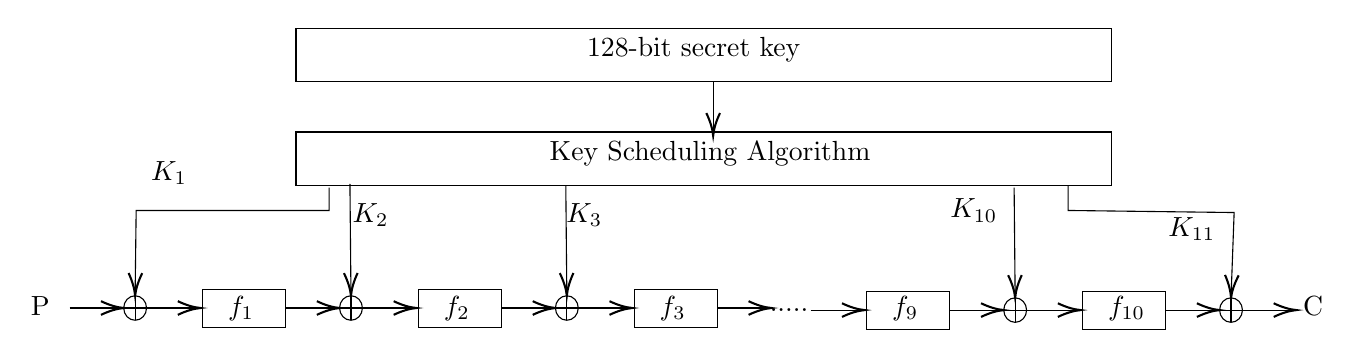
\begin{tikzpicture}[x=0.75pt,y=0.75pt,yscale=-1,xscale=1]
        \draw   (146,38) -- (539,38) -- (539,63.8) -- (146,63.8) -- cycle ;
        \draw    (347,63.8) -- (347,87.8) ;
        \draw [shift={(347,89.8)}, rotate = 270] [color={rgb, 255:red, 0; green, 0; blue, 0 }  ][line width=0.75]    (10.93,-3.29) .. controls (6.95,-1.4) and (3.31,-0.3) .. (0,0) .. controls (3.31,0.3) and (6.95,1.4) .. (10.93,3.29)   ; 
        \draw   (146,88) -- (539,88) -- (539,113.8) -- (146,113.8) -- cycle ;
        \draw    (37,172.8) -- (61,172.8) ;
        \draw [shift={(63,172.8)}, rotate = 180] [color={rgb, 255:red, 0; green, 0; blue, 0 }  ][line width=0.75]    (10.93,-3.29) .. controls (6.95,-1.4) and (3.31,-0.3) .. (0,0) .. controls (3.31,0.3) and (6.95,1.4) .. (10.93,3.29)   ;
        \draw   (63,172.8) .. controls (63,169.54) and (65.46,166.9) .. (68.5,166.9) .. controls (71.54,166.9) and (74,169.54) .. (74,172.8) .. controls (74,176.06) and (71.54,178.7) .. (68.5,178.7) .. controls (65.46,178.7) and (63,176.06) .. (63,172.8) -- cycle ; \draw   (63,172.8) -- (74,172.8) ; \draw   (68.5,166.9) -- (68.5,178.7) ;
        \draw    (74,172.8) -- (98,172.8) ;
        \draw [shift={(100,172.8)}, rotate = 180] [color={rgb, 255:red, 0; green, 0; blue, 0 }  ][line width=0.75]    (10.93,-3.29) .. controls (6.95,-1.4) and (3.31,-0.3) .. (0,0) .. controls (3.31,0.3) and (6.95,1.4) .. (10.93,3.29)   ;
        \draw   (101,163.8) -- (141,163.8) -- (141,182) -- (101,182) -- cycle ;
        \draw    (141,172.8) -- (165,172.8) ;
        \draw [shift={(167,172.8)}, rotate = 180] [color={rgb, 255:red, 0; green, 0; blue, 0 }  ][line width=0.75]    (10.93,-3.29) .. controls (6.95,-1.4) and (3.31,-0.3) .. (0,0) .. controls (3.31,0.3) and (6.95,1.4) .. (10.93,3.29)   ;
        \draw   (167,172.8) .. controls (167,169.54) and (169.46,166.9) .. (172.5,166.9) .. controls (175.54,166.9) and (178,169.54) .. (178,172.8) .. controls (178,176.06) and (175.54,178.7) .. (172.5,178.7) .. controls (169.46,178.7) and (167,176.06) .. (167,172.8) -- cycle ; \draw   (167,172.8) -- (178,172.8) ; \draw   (172.5,166.9) -- (172.5,178.7) ;
        \draw    (178,172.8) -- (202,172.8) ;
        \draw [shift={(204,172.8)}, rotate = 180] [color={rgb, 255:red, 0; green, 0; blue, 0 }  ][line width=0.75]    (10.93,-3.29) .. controls (6.95,-1.4) and (3.31,-0.3) .. (0,0) .. controls (3.31,0.3) and (6.95,1.4) .. (10.93,3.29)   ; 
        \draw   (205,163.8) -- (245,163.8) -- (245,182) -- (205,182) -- cycle ; 
        \draw    (245,172.8) -- (269,172.8) ;
        \draw [shift={(271,172.8)}, rotate = 180] [color={rgb, 255:red, 0; green, 0; blue, 0 }  ][line width=0.75]    (10.93,-3.29) .. controls (6.95,-1.4) and (3.31,-0.3) .. (0,0) .. controls (3.31,0.3) and (6.95,1.4) .. (10.93,3.29)   ; 
        \draw   (271,172.8) .. controls (271,169.54) and (273.46,166.9) .. (276.5,166.9) .. controls (279.54,166.9) and (282,169.54) .. (282,172.8) .. controls (282,176.06) and (279.54,178.7) .. (276.5,178.7) .. controls (273.46,178.7) and (271,176.06) .. (271,172.8) -- cycle ; \draw   (271,172.8) -- (282,172.8) ; \draw   (276.5,166.9) -- (276.5,178.7) ;
        \draw    (282,172.8) -- (306,172.8) ;
        \draw [shift={(308,172.8)}, rotate = 180] [color={rgb, 255:red, 0; green, 0; blue, 0 }  ][line width=0.75]    (10.93,-3.29) .. controls (6.95,-1.4) and (3.31,-0.3) .. (0,0) .. controls (3.31,0.3) and (6.95,1.4) .. (10.93,3.29)   ;
        \draw   (309,163.8) -- (349,163.8) -- (349,182) -- (309,182) -- cycle ;
        \draw    (349,172.8) -- (373,172.8) ;
        \draw [shift={(375,172.8)}, rotate = 180] [color={rgb, 255:red, 0; green, 0; blue, 0 }  ][line width=0.75]    (10.93,-3.29) .. controls (6.95,-1.4) and (3.31,-0.3) .. (0,0) .. controls (3.31,0.3) and (6.95,1.4) .. (10.93,3.29)   ;
        \draw    (394,173.8) -- (418,173.8) ;
        \draw [shift={(420,173.8)}, rotate = 180] [color={rgb, 255:red, 0; green, 0; blue, 0 }  ][line width=0.75]    (10.93,-3.29) .. controls (6.95,-1.4) and (3.31,-0.3) .. (0,0) .. controls (3.31,0.3) and (6.95,1.4) .. (10.93,3.29)   ;
        \draw   (421,164.8) -- (461,164.8) -- (461,183) -- (421,183) -- cycle ;
        \draw    (461,173.8) -- (485,173.8) ;
        \draw [shift={(487,173.8)}, rotate = 180] [color={rgb, 255:red, 0; green, 0; blue, 0 }  ][line width=0.75]    (10.93,-3.29) .. controls (6.95,-1.4) and (3.31,-0.3) .. (0,0) .. controls (3.31,0.3) and (6.95,1.4) .. (10.93,3.29)   ;
        \draw   (487,173.8) .. controls (487,170.54) and (489.46,167.9) .. (492.5,167.9) .. controls (495.54,167.9) and (498,170.54) .. (498,173.8) .. controls (498,177.06) and (495.54,179.7) .. (492.5,179.7) .. controls (489.46,179.7) and (487,177.06) .. (487,173.8) -- cycle ; \draw   (487,173.8) -- (498,173.8) ; \draw   (492.5,167.9) -- (492.5,179.7) ;
        \draw    (498,173.8) -- (522,173.8) ;
        \draw [shift={(524,173.8)}, rotate = 180] [color={rgb, 255:red, 0; green, 0; blue, 0 }  ][line width=0.75]    (10.93,-3.29) .. controls (6.95,-1.4) and (3.31,-0.3) .. (0,0) .. controls (3.31,0.3) and (6.95,1.4) .. (10.93,3.29)   ;
        \draw   (525,164.8) -- (565,164.8) -- (565,183) -- (525,183) -- cycle ;
        \draw    (565,173.8) -- (589,173.8) ;
        \draw [shift={(591,173.8)}, rotate = 180] [color={rgb, 255:red, 0; green, 0; blue, 0 }  ][line width=0.75]    (10.93,-3.29) .. controls (6.95,-1.4) and (3.31,-0.3) .. (0,0) .. controls (3.31,0.3) and (6.95,1.4) .. (10.93,3.29)   ;
        \draw   (591,173.8) .. controls (591,170.54) and (593.46,167.9) .. (596.5,167.9) .. controls (599.54,167.9) and (602,170.54) .. (602,173.8) .. controls (602,177.06) and (599.54,179.7) .. (596.5,179.7) .. controls (593.46,179.7) and (591,177.06) .. (591,173.8) -- cycle ; \draw   (591,173.8) -- (602,173.8) ; \draw   (596.5,167.9) -- (596.5,179.7) ; 
        \draw    (602,173.8) -- (626,173.8) ;
        \draw [shift={(628,173.8)}, rotate = 180] [color={rgb, 255:red, 0; green, 0; blue, 0 }  ][line width=0.75]    (10.93,-3.29) .. controls (6.95,-1.4) and (3.31,-0.3) .. (0,0) .. controls (3.31,0.3) and (6.95,1.4) .. (10.93,3.29)   ;
        \draw    (162,114.8) -- (162,125.8) -- (69,125.8) -- (68.52,164.9) ;
        \draw [shift={(68.5,166.9)}, rotate = 270.7] [color={rgb, 255:red, 0; green, 0; blue, 0 }  ][line width=0.75]    (10.93,-3.29) .. controls (6.95,-1.4) and (3.31,-0.3) .. (0,0) .. controls (3.31,0.3) and (6.95,1.4) .. (10.93,3.29)   ;
        \draw    (172,113) -- (172.48,164.9) ;
        \draw [shift={(172.5,166.9)}, rotate = 269.47] [color={rgb, 255:red, 0; green, 0; blue, 0 }  ][line width=0.75]    (10.93,-3.29) .. controls (6.95,-1.4) and (3.31,-0.3) .. (0,0) .. controls (3.31,0.3) and (6.95,1.4) .. (10.93,3.29)   ;
        \draw    (276,113.8) -- (276.48,164.9) ;
        \draw [shift={(276.5,166.9)}, rotate = 269.46] [color={rgb, 255:red, 0; green, 0; blue, 0 }  ][line width=0.75]    (10.93,-3.29) .. controls (6.95,-1.4) and (3.31,-0.3) .. (0,0) .. controls (3.31,0.3) and (6.95,1.4) .. (10.93,3.29)   ;
        \draw    (492,114.8) -- (492.48,165.9) ;
        \draw [shift={(492.5,167.9)}, rotate = 269.46] [color={rgb, 255:red, 0; green, 0; blue, 0 }  ][line width=0.75]    (10.93,-3.29) .. controls (6.95,-1.4) and (3.31,-0.3) .. (0,0) .. controls (3.31,0.3) and (6.95,1.4) .. (10.93,3.29)   ;
        \draw    (518,113.8) -- (518,125.8) -- (598,126.8) -- (596.57,165.9) ;
        \draw [shift={(596.5,167.9)}, rotate = 272.09] [color={rgb, 255:red, 0; green, 0; blue, 0 }  ][line width=0.75]    (10.93,-3.29) .. controls (6.95,-1.4) and (3.31,-0.3) .. (0,0) .. controls (3.31,0.3) and (6.95,1.4) .. (10.93,3.29)   ;
        
        \draw (285,41) node [anchor=north west][inner sep=0.75pt]   [align=left] {128-bit secret key};
        \draw (267,91) node [anchor=north west][inner sep=0.75pt]   [align=left] {Key Scheduling Algorithm};
        \draw (17,166) node [anchor=north west][inner sep=0.75pt]   [align=left] {P};
        \draw (112,166) node [anchor=north west][inner sep=0.75pt]   [align=left] {$f_1$};
        \draw (216,166) node [anchor=north west][inner sep=0.75pt]   [align=left] {$f_2$};
        \draw (320,166) node [anchor=north west][inner sep=0.75pt]   [align=left] {$f_3$};
        \draw (373,172) node [anchor=north west][inner sep=0.75pt]   [align=left] {.....};
        \draw (432,166) node [anchor=north west][inner sep=0.75pt]   [align=left] {$f_9$};
        \draw (536,166) node [anchor=north west][inner sep=0.75pt]   [align=left] {$f_{10}$};
        \draw (630,166) node [anchor=north west][inner sep=0.75pt]   [align=left] {C};
        \draw (75,101) node [anchor=north west][inner sep=0.75pt]   [align=left] {$K_1$};
        \draw (172,121) node [anchor=north west][inner sep=0.75pt]   [align=left] {$K_2$};
        \draw (275,121) node [anchor=north west][inner sep=0.75pt]   [align=left] {$K_3$};
        \draw (460,119) node [anchor=north west][inner sep=0.75pt]   [align=left] {$K_{10}$};
        \draw (565,128) node [anchor=north west][inner sep=0.75pt]   [align=left] {$K_{11}$};
    \end{tikzpicture}
\end{center}

\end{document}